\chapter{Design of propulsion systems}
\section{System conceptualization}
\section{Subsystem design}
\subsection{Regenerative cooling}
\subsection{Catalyzer}
\subsection{Injectors}
\subsection{Feeding system}
After having designed most of our propulsion system. We need to carefully link them by designing our feeding system. The biggest challenge is to create a system that will both fit in our spacecraft and deliver the right amount of propellant from the tanks to the engine through our different, required other subsystems.\\

The general pressure loss in a system is given by :

$$
\Delta P = K\frac \rho 2 w^2
$$

With $K$ depending on the type of change in system geometry as follow : 
\begin{figure}[H]
	\centering
	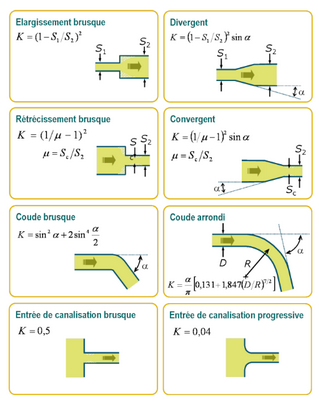
\includegraphics[height=12cm]{pertecharge}
	\caption{$K$ values for geometry changes}
\end{figure}
In our case, we will use the progressive line entering loss $K = 0.04$ and the bends $ K(\alpha) = \sin^2(\alpha) + 2\sin^4\bigg(\frac\alpha 2\bigg)$. Another $K$ will also be used for the entrance of the injector, which will be specified later on.\\

For manufacturing costs and simplicity purposes, we choose to only use $45^\circ$ bends which will result in $K_{bends}=0.5429$.\\

With that and the length measurements in mind, we designed the following feeding system layout for which we will then calculate the pressure variations along it :
\begin{figure}[H]
	\centering
	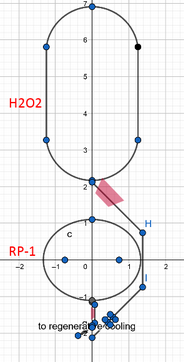
\includegraphics[height=10cm]{feeding}
	\caption{Feeding system layout (To scale)}
\end{figure}
\begin{figure}[H]
	\centering
	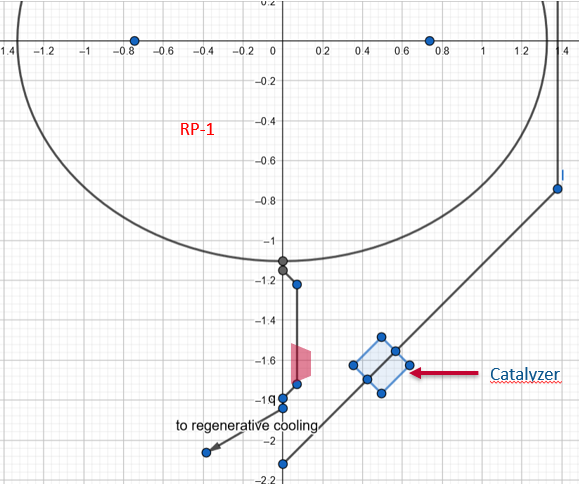
\includegraphics[height=8cm]{feedingzoom}
	\caption{Feeding system layout - Zoomed (To scale)}
\end{figure}
\subsubsection{Line diameters}
In order to choose our line diameters, we can first use our volume flow and then get the line area from it and then at the end, the line diameter.\\
\underline{Fuel} 
\begin{align}
\dot{V_f}&= \frac{\dot{m_f}}{\rho_f} = 0.0015298m^3/s\\
A_{line_f} &= \frac{\dot V_f}{w_f}=5.21\times 10^{-5} mm^2\\
d_{line_f} &= 2\sqrt{\frac{A_{line_f}}{\pi}} = 8.1447mm
\end{align}
As we are trying to insure a high injection velocity and to insure a certain margin in pressure and velocity, we will choose a line diameter of $7$ mm for the fuel feeding system.
\underline{Oxidizer}
\begin{align}
\dot{V_o}&= \frac{\dot{m_o}}{\rho_o} = 0.006042m^3/s\\
A_{line_o} &= \frac{\dot V_o}{w_o}=0.000275 mm^2\\
d_{line_o} &= 2\sqrt{\frac{A_{line_o}}{\pi}} = 18mm
\end{align}
In this case, we will choose a line diameter of $15$ mm for the oxidizer.

\subsubsection{Fuel feeding system}
The following items in our fuel feeding system will cause pressure drops :
\begin{itemize}
	\item Tank exit : $K=0.04$
	\item 4 $\times$ $45^\circ$ bends : $K = 0.5429$ for each
	\item Straight line losses : $\Delta P = \frac \rho 2 w^2 f \frac{L}{D}$
	\item Friction coefficient : $f = 0.02$
	\item Regenerative cooling : $\Delta P = 0.25$ bar
	\item Fuel injection : $\Delta P = 9.3843$ bars
\end{itemize}

With our current layout, we have $5$ straight lines which will cause pressure losses on the fuel side. Three of them are before the turbopump which is placed at the end of the third straight section, right before the third bend. We consider a velocity of $8$ m/s before the turbopumps and of $v_{inj}=29.363$ m/s after. The line loss for each section is given by : 
$$
\Delta P = \frac {810} 2 w^2 \times 0.02 \times \frac{L_{section}}{0.007}
$$
\begin{enumerate}
	\item First section ($L_{section}=0.05m$) : $\Delta P = 0.037029$ bar
	\item Second section ($L_{section}=0.1m$) : $\Delta P = 0.074057$ bar
	\item Third section ($L_{section}=0.5m$) : $\Delta P = 0.37029$ bar
	\item Fourth section ($L_{section}=0.1m$) : $\Delta P = 0.997699$ bar
	\item Fifth section ($L_{section}=0.05m$) : $\Delta P = 0.49884$ bar
\end{enumerate}
There are also two different values for the bend losses depending on the position of the bend (before or after the turbopump), we have $2$ of each :
\begin{itemize}
	\item $\Delta P_{before} = 0.14072 $ bar
	\item $\Delta P_{after} = 1.8957$ bar
\end{itemize}
The tank exit loss is :
$$
\Delta P_{exit} = K_{exit} \times \frac{\rho_F}2 \times 8 ^ 2 = 0.010368\text{ bar}
$$
\subsubsection{Oxidizer feeding system}
The following items in our oxidizer feeding system will cause pressure drops :
\begin{itemize}
	\item Tank exit : $K=0.04$
	\item 4 $\times$ $45^\circ$ bends : $K = 0.5429$ for each
	\item Straight line losses : $\Delta P = \frac \rho 2 w^2 f \frac{L}{D}$
	\item Friction coefficient : $f = 0.02$
	\item Catalyzer : $\Delta P = $ bars
	\item Oxidizer injection : $\Delta P = 4.9599$ bars
\end{itemize}

On this part of the feeding system, we also have $5$ sections and $4$ bends of $45^\circ$ each. We also consider a velocity of $8$ m/s before the turbopump and $21.971$ m/s after. However, due to the larger distances (due to our tank layout), the turbopump's position in the feeding system is different and is now positioned after the first bend, right at the beginning of the second straight line. This results in $3$ bends being at high velocity and $1$ at relatively slower velocity.\\

Here, each straight line loss section is given by : 
$$
\Delta P = \frac {1450} 2 w^2 \times 0.02 \times \frac{L_{section}}{0.015}
$$
With : 

\begin{enumerate}
	\item First section ($L_{section}=0.05m$) : $\Delta P = 0.030933$ bar
	\item Second section ($L_{section}=1.95m$) : $\Delta P = 9.0992$ bars
	\item Third section ($L_{section}=1.4836m$) : $\Delta P = 6.9228$ bars
	\item Fourth section ($L_{section}=1.15m$) : $\Delta P = 5.3662$ bars
	\item Fifth section ($L_{section}=0.6m$) : $\Delta P = 2.7997$ bars
\end{enumerate}

For the bends, we have :

\begin{itemize}
	\item $\Delta P_{before} = 0.2519 $ bar ($1$ of them)
	\item $\Delta P_{after} = 1.0614$ bar ($3$ of them)
\end{itemize}

The tank exit loss is :
$$
\Delta P_{exit} = K_{exit} \times \frac{\rho_o}2 \times 8 ^ 2 = 0.01856\text{ bar}
$$
\subsection{Turbo pumps}
As most of our subsystems have a defined pressure drop due to their specific design, we have made the choice to use this feeding system design with all losses included to then design our turbopumps to have a pressure rise in accordance with our pressure requirements. We chose to go with electrically driven turbo pumps as we have a good amount of electrical power since we use fuel cells in our spacecraft.\\

Our respective turbopump required created pressures are : 
\begin{itemize}
	\item Fuel side : $\Delta P_{T_f} = P_{Chamber} + \Delta P_{feeding_f} + \Delta P_{inj_f} + \Delta P_{Regenerative\ cooling} - P_{Tank_f}$
	\item Oxidizer side : 	$\Delta P_{T_o} = P_{Chamber} + \Delta P_{feeding_o} + \Delta P_{inj_o} + \Delta P_{Catalyzer} - P_{Tank_o}$
\end{itemize}
Thus,
\begin{align}
	\Delta P_{T_f} &= 54.395\ \text{bars}\\
	\Delta P_{T_o} &= 102.28\ \text{bars}
\end{align}
\subsection{Pressure evolution summary}
\subsubsection{Fuel side}
\begin{tabular}[H]{|c|c|c|}
	\hline
	\cellcolor{gray!50}Contributor& \cellcolor{gray!50}Pressure Drop (bars) & \cellcolor{gray!50}Pressure at the end of this part (bars)\\
	\hline
	Tank & NA & $1.3$ \\
	\hline
	Tank exit & $0.010368$ & $1.29$\\
	\hline
	First section & $0.037$ &$1.253$\\
	\hline
	First bend &$0.14$ &$1.113$\\
	\hline
	Second section &$0.074$ &$1.039$\\
	\hline
	Second bend &$0.14$ &$0.899$\\
	\hline
	Third section &$0.37$ &$0.529$\\
	\hline
	Turbo pump & $54.395 $ (Rise) &$54.924$\\
	\hline
	Third bend &$1.8957$ &$53.0283$\\
	\hline
	Fourth section &$0.997$ &$52.0313$\\
	\hline
	Fourth bend &$1.8957$ &$50.1356$\\
	\hline
	Fifth section &$0.499$ &$49.6366$\\
	\hline
	Cooling &$0.25$ &$49.3866$\\
	\hline
	Injection &$9.38$ &$40.0066$\\
	\hline
	Combustion chamber & NA &$40.0066$\\
	\hline
\end{tabular}
\begin{figure}[H]
	\centering
	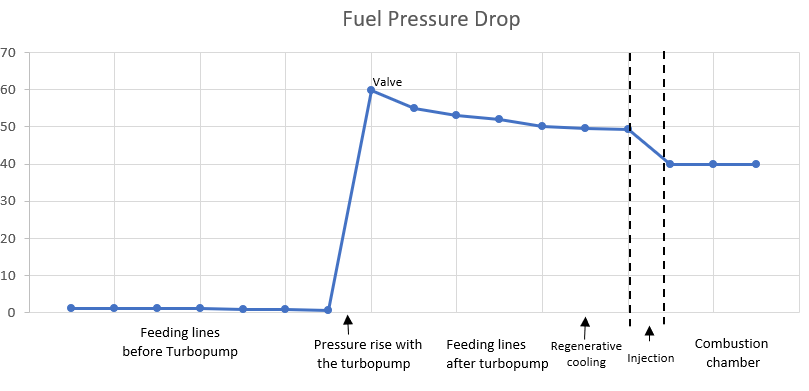
\includegraphics[width=\linewidth]{fuelchart}
	\caption{Pressure evolution on fuel side (bars)}
\end{figure}
\subsubsection{Oxidizer side}
\begin{tabular}[H]{|c|c|c|}
	\hline
	\cellcolor{gray!50}Contributor& \cellcolor{gray!50}Pressure Drop (bars) & \cellcolor{gray!50}Pressure at the end of this part (bars)\\
	\hline
	Tank & NA & $1.3$ \\
	\hline
	Tank exit & $0.010368$ & $1.29$\\
	\hline
	First section & $0.031$ &$1.259$\\
	\hline
	First bend &$0.25$ &$1.009$\\
	\hline
	Turbo pump & $102.28 $ (Rise) &$103.289$\\
	\hline
	Second section &$9.09$ &$94.199$\\
	\hline
	Second bend &$1.06$ &$93.139$\\
	\hline
	Third section &$6.9228$ &$86.2162$\\
	\hline
	Third bend &$1.06$ &$85.1562$\\
	\hline
	Fourth section &$5.366$ &$79.7902$\\
	\hline
	Fourth bend &$1.06$ &$78.7302$\\
	\hline
	Fifth section &$2.7997$ &$75.9305$\\
	\hline
	Catalyzer &$30.95$ &$44.9805$\\
	\hline
	Injection &$4.96$ &$40.0205$\\
	\hline
	Combustion chamber & NA &$40.0205$\\
	\hline
\end{tabular}

\begin{figure}[H]
	\centering
	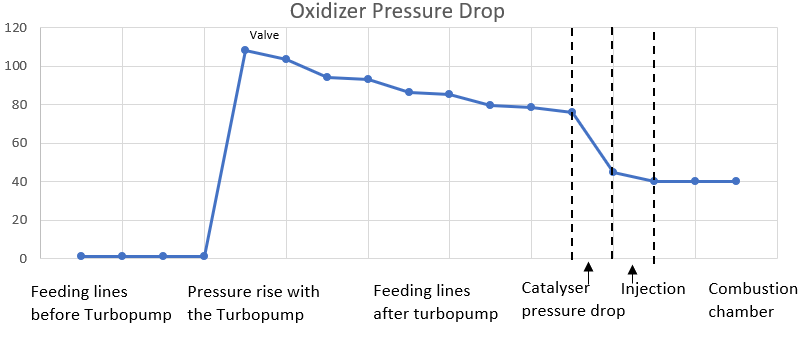
\includegraphics[width=\linewidth]{oxchart}
	\caption{Pressure evolution on oxidizer side (bars)}
\end{figure}
\section{Design review}
